\documentclass[11pt, openany]{book}              % Book class in 11 points
\parindent0pt  \parskip10pt             % make block paragraphs
\raggedright                            % do not right justify

\usepackage{amsmath,amsfonts,amssymb,amsthm}
\usepackage{mathtools}
\usepackage{commath}
\usepackage[sc,osf]{mathpazo}

\let\oldnorm\norm   % <-- Store original \norm as \oldnorm
\let\norm\undefined % <-- "Undefine" \norm
\DeclarePairedDelimiter\norm{\lVert}{\rVert}
\DeclareMathOperator*{\argmax}{arg\,max}  % in your preamble
\DeclareMathOperator*{\argmin}{arg\,min}  % in your preamble 

\title{\bf Machine Learning Handbook}    % Supply information
\author{Xinhe Liu}              %   for the title page.
\date{2018-2-28}                           %   Use current date. 

% Note that book class by default is formatted to be printed back-to-back.
\begin{document}                        % End of preamble, start of text.
% \frontmatter                            % only in book class (roman page #s)
\maketitle                              % Print title page.
\tableofcontents                        % Print table of contents
\mainmatter                             % only in book class (arabic page #s)

\part{High-level Views}
\chapter{Math Review}

\section{Linear Algebra}

Concepts:

\begin{itemize}
    \item scalar, vector, matrix, tensor(n-rank tensor, matrix is a rank 2 tensor) 
    \item Gaussian Elimination, rank
    \item p-norm $$|X|_p = (\sum_i |x_i|^p)^{\frac{1}{p}}$$
    \item inner product$<x_i,y_i>$, outer product
    \item orthogonal,dimension, basis, orthogonal basis
    \item linear transformation $Ax = y$
    \item eigenvalue, eigenvector $Ax =\lambda x$ (transformation and speed)
    \item vector space, linear space(with summation, scalar production), inner product space( inner product space) 
\end{itemize}


\section{Probability}

Concepts:

\begin{itemize}
    \item Classic Probability Model: Frequentist 
    \item Bayesian Probability Theory 
    \item Random variable, continuous RV, discrete RV, probability mass function, probability density function, cumulative density function
    \item expectation, moments, variance, covariance, correlation coefficient
\end{itemize}


Theorems:

\begin{itemize}
    \item Law of Total Probability
    \item Bayes' Rule $$P(H|D) = \frac{P(D|H) P(H)}{P(D)}$$ $P(H)$-prior probability, $P(D|H)$-likelihood, $P(H|D)$-posterior probability,
\end{itemize}

Important Distributions: 

\begin{enumerate}
	\item Bernoulli distribution
	\item Binomial distribution(n,p)$$P(X=k) = {N\choose k} p^k (1-p)^{(n-k)}$$
	\item Poisson distribution $$P(X=k) = \lambda^k \frac{e^{-\lambda}}{k!}$$
	\item Normal Distribution, See next chapter
	\item Bernoulli Distribution 
	\item Uniform Distribution,
	\item Exponential distribution $$e^{-\frac{x}{\theta}}\theta$$ $$P(x>s+t|X>s) = P(x>t)$$, 
	\item Poisson Distribution
	\item normal distribution
	\item t-distribution	
\end{enumerate} 

Moment Generating Functions:

\section{Information Theory}

Concepts:

\begin{itemize}
    \item Information $$h(A) = -log_2 p(A)$$ (bit)
    \item (Information Source) Entropy $$ H(X) = -\sum_{i=1}^n p(a_i)log_2p(a_i) \leq log_2 n$$ Maximize under equal probability
    \item Conditional Entropy $$H(Y|X)  = -\sum_{i=1}^n p(x_i)H(Y|X=x_i)= -\sum_{i=1}^n p(x_i)\sum_{j=1}^n p(y_j|x_i) log_2p(y_j|x_i) $$ $$ = \sum_{i=1}^n \sum_{j=1}^n p(x_i,y_j) log_2p(y_j|x_i) $$
    \item Mutual Information/Information Gain $$I(X;Y) = H(Y) - H(Y|X)$$
    \item Kullback-Leibler Divergence (K-L) Divergence 
      $$D_{KL}(P||Q) = \sum_{i=1}^n p(x_i) log_2\frac{p(x_i)}{q(x_i)} \neq D_{KL}(Q||P)$$
      $$D_{KL}(f,\hat{f})) = \int_{-\infty}^{\infty} log(\frac{f_X(x)}{\hat{f(x)}})f_X(x)dx $$
     K-L Divergence Measures the Distance of two distributions. The optimal encoding of information has the same bits as the entropy. Measures the extra bits if the real distribution is q rather than p. (Using P to approximate Q) K-L divergence plays an important role in both information theory and MLE theory. MLE $\hat{\theta}$ is actually finding the closest K-L Distance approximation of $f(x;\theta)$ to sample distribution.
\end{itemize}
Theorems:

\begin{itemize}
    \item The Maximum Entropy Principle. Without extra assumption, max entropy/equal probability has the minimum prediction risk. 
\end{itemize}
 
\section{Optimization}

\subsection{Optimization Theory}

\begin{itemize}
    \item Objective function/Evaluation function, constrained/unconstrained optimization,Feasible Set, Optimal Solution, Optimal Value, Binding Constraints, Shadow Price, Infeasible Price, Infeasibility, Unboundedness    
    \item Linear Programming
    \item Lagrange Multiplier $$L(x,y,\lambda) = f(x,y) + \lambda \varphi(x,y) $$
    \item Convex Set, Convex Function $f:S\to R$ is convex if and only if $\bigtriangledown^2 f(\mathbf{x})$ is positive semidefinite 
\end{itemize}

\subsection{Optimization Methods}

\begin{itemize}
    \item Linear Search Method: Direction First, Step Size second	
    	\begin{itemize}  		
    		\item Gradient Descent: Batch Processing(Use all samples) vs Stochastic Gradient Descent(Use one sample)
    		$$ \theta = \theta - \alpha \frac{\partial J }{ \partial \theta }$$
    		\item Newton's Method: Use Curvature Information 
    		$$ \mathbold{\beta}^{t+1} = \mathbold{\beta}^t - (\frac{\partial^2 Loss(\mathbold{\beta})}{\partial \mathbold{\beta} \partial\mathbold{\beta}^T})^{-1} \frac{ \partial Loss(\mathbold{\beta})}{\partial \mathbold{\beta}} $$
   		\end{itemize}
   	\item Trust Region: Step first, direction second. Find optimal direction of second-order approximation. If the descent size is too small, make step size smaller.
   	\item Heuristics Method
   		\begin{itemize}  		
	    	\item Genetic Algorithm
	 	   	\item Simulated Annealing 
	    	\item Partical Swarming/Ant Colony Algorithm
	    \end{itemize}
\end{itemize}

Quadratic programming (QP)

\begin{itemize}
    \item Sequential Minimal Optimization(SMO) 
\end{itemize}

\subsection{Optimization Algorithms in Machine Learning}

		Loss Function
			Entropy
			K-L Distance
		Regularization Methods
		EM Algorithm
		Gradient Descent
			Stochastic Gradient Descent
			Batch Gradient Descent
			Momentum
			AdaGrad
			Adam
		Backward Propagation
		Gradient Checkling
		
\subsection{Optimization in Deep Learning}

Optimization Algos used in Deep Learning Includes

\begin{itemize}
	\item Mini-batch gradient descent: Use one batch (subset) of sample to compute the gradient each time. ( one “epoch”) ( one batch size =1, it is Stochastic gradient descent)
	\item Momentum Method: Smooth the gradient series with EWMA (Exponentially weighted averages 
	$$ V_{dw} = \beta_1V_{dw} + (1-\beta_1) dw, V_{dw} /= (1-\beta_1^t)$$
 	$$ V_{db} = \beta_1V_{db} + (1-\beta_1) dw,V_{db} /= (1-\beta_1^t)$$
 	\item Root-Mean Square Prop (RMSProp)
 	$$ S_{dw} = \beta S_{dw} + (1-\beta) dw^2 $$
 	$$ S_{db} = \beta S_{db} + (1-\beta) dw^2 $$
	$$ w:= w- \alpha \frac{dw}{\sqrt{sdw}}, b:= b- \alpha \frac{db}{\sqrt{sdb}}$$
	\item Adam(Adaptive Moment Estimation) Algorithm L Combine RMSProp and Momentum
	$$ V_{dw} = \beta_1V_{dw} + (1-\beta_1) dw, V_{dw} /= (1-\beta_1^t)$$
 	$$ V_{db} = \beta_1V_{db} + (1-\beta_1) dw,V_{db} /= (1-\beta_1^t)$$
 	$$ S_{dw} = \beta_2S_{dw} + (1-\beta_2) dw^2 $$
 	$$ S_{db} = \beta_2S_{db} + (1-\beta_2) dw^2 $$
	$$w:= w- \alpha \frac{v_{dw}}{\sqrt{sdw}+\epsilon}, b:= b- \alpha \frac{v_{db}}{\sqrt{sdb}+\epsilon}$$
	$$w:= w- \alpha \frac{dw}{\sqrt{sdb}+\epsilon}, b:= b- \alpha \frac{db}{\sqrt{sdb}+\epsilon}$$
	\item Learning Rate Decay
		$$ \alpha = \frac{1}{1+\text{decay rate} \times \text{epoch num}}$$	
\end{itemize}

\subsection{Hyperparameter Tuning Methods}

\begin{itemize}
	\item Grid method 
	\item Batch Normalization 
	$$z_{norm} = \frac{z^{(i)}-\mu}{\sqrt{\sigma^2 + \epsilon}}$$
	$$\tilde{z} = \gamma z_{norm}  + \beta$$
	Can speed up learning and add some noise to avoid overfitting. (Similar to dropout).
	In test time, usually use the EWMA across mini-batches on the mean and variance series to normalize the use trained $\beta, \gamma$ to transform. 
\end{itemize}

\section{Formal Logic}

Concepts
\begin{itemize}
    \item Generative Expert System: Rule+Facts+Deduction Engine 
    \item Godel's incompleteness theorems
\end{itemize}

\chapter{Statistics}

\section{Concepts}
\subsection{Basic}
\begin{itemize}
    \item parameter(constant for probability model), statistic (model of sample data), data, sample, population
    \item point estimation, interval estimation, Confidence Interval( $P(L \leq \theta \leq U )$, notice: $\theta$ is not random, L, U is random! ( We repeat constructing confidence interval a n times, $\alpha$ percent of the times, it will contain $theta$.
\end{itemize}

\subsection{Estimator and Estimation}

\begin{itemize}
    \item Method of Moments: $E(X^k)$ based on LOLN.\\ 
    	If We have p parameters, we can use p moments to form a system of equations to solve $\theta_1,...\theta_p$
    	$$\sum_{i=1}^n X_i^j= E(X^j)$$, for j = 1,...,p
    \item Maximum Likelihood Estimation. Multiply p.m.f/p.d.f since every sample is independent. Maximize the likelihood of finding samples. \\ If $X_1,...X_n \stackrel{i.i.d}{\sim} f_x(x, \theta)$, 
    	$$ l(\theta) =  \prod_{i=1}^n f_{X_i} (x_i; \theta), L(\theta ) = log l(\theta)$$
    	$$ \hat{\theta}_{MLE}= argmax_{\theta} f_x(x;\theta ) = argmax_{\theta} L(\theta )$$
    	Analytical or Numerically solved. $$ \frac{\partial}{\partial \theta} [log L(\theta ) ] = 0, \frac{\partial^2}{\partial \theta^2} [log L(\theta ) ] < 0$$, for multiple parameters, we need the Hessian matrix to be negative definite $x^tHx<0, \forall x$ 
    	
    \item Properties of MLE
    	\begin{enumerate}
    		\item Invariance $\hat{\theta}$ is MLE of $\theta$, then $g(\hat{\theta})$ is MLE of $g(\theta)$
    		\item Consistency $$P(\hat{\theta} - \theta ) \rightarrow 0$$ as $n \rightarrow 0, \forall \epsilon > 0$ Under the conditions
    		\begin{enumerate}
    			\item $X_1,...X_n \stackrel{i.i.d}{\sim} f_x(x|\theta)$
    			\item parameters are identifiable, $\theta \neq \theta', f_x(x|\theta) \neq f_x(x|\theta')$
    			\item densities $f_x(x|\theta)$ has common support(set of x with positive density/probability), $f_x(x|\theta)$ is differentiable at $\theta$
    			\item parameter space $\Omega$ contains open set $\omega$ where true $\theta_0$ is an interior point
    		\end{enumerate}
    		\item Asymptotic Normality 
    		$$ \sqrt{n}(\hat{\theta}_{MLE} - \theta_0) \rightarrow N(0, I^{-1}(\theta_0)) $$
    		$$ I(\theta_0) = E( -(\frac{\partial}{\partial \theta} [log f(x, \theta ) ])^2)=E(-\frac{\partial^2}{\partial \theta^2} [log f(x, \theta ) ] )$$ 
    		called the Fisher Information
    		$$ \hat{\theta}_{MLE} \approx N(\theta_0, \frac{1}{n I(\theta_0)})$$
    		$$ n I(\theta_0) = E( -\frac{\partial^2}{\partial \theta^2} log L(\theta) )$$
    		\begin{itemize}
    		\item	So the Variance of MLE( $1/ E( -\frac{\partial^2}{\partial \theta^2} log L(\theta) )$) is the reciprocal of amount of curvature at MLE. 
    			Usually, We can just use the \textit{observed Fisher Information} (curvature near $\hat{\theta_{MLE}}$) instead. ($I(\hat{\theta_{MLE}})$) \\
    		$\frac{1}{ n I(\theta_0)}$ is called Cramer-Rao Lower Bound. \\ Under Multi-dimensional Case, 
    		
    			$$ I(\theta_0)_{ij} = =E(-\frac{\partial^2}{\partial \theta_i \partial \theta_j} [log f(x, \theta ) ] )$$ $Hessian \approx nI(\theta_0)$ $Hessian^{-1} \approx nI(\theta_0)$ when we use numerical approach. 

    		\item Under the above four conditions plus 
    			\begin{enumerate}
    				\item $ \forall x \in \chi$, $f_x(x|\theta)$ is three times differentiable with respect to $\theta$, and third derivative is continuous at $\theta$, and $\int f_x(x|\theta) dx$ can be differentiated three times under integral sign
    				\item $ \forall \theta \in \Omega, \exists c, M(x)$ (both depends on $\theta_0$) such that
    				$$ \frac{\partial^3}{\partial \theta^3} [log f(x, \theta ) ] \leq M(x), \forall x \in \chi, \theta_0-c<\theta < \theta_0+c, E_{\theta_0} [M(x)] < \infty$$
    			\end{enumerate}
    		\end{itemize}
    	\end{enumerate}
    	
    \item $\Delta$ -Method: $g(\hat{theta}_{MLE})$ is approximately
    	  $$ N(g(\theta), (g'(\theta))^2 \frac{1}{nI(\theta)})$$ if asymptotic normality is satisfied. \\
    	  In Multivariate Case:
    	  $$ \hat{\theta} \sim N(\theta, \Sigma/n), \theta,\hat{\theta} \in R^p $$
    	  $$g: R^p \rightarrow R^m$$
    	  $$g(\hat{\theta}) \sim N(g(\theta), G\Sigma G^T/n)$$
		  $$ G = \begin{pmatrix} 
  				\frac{\partial{g_1(\theta)}}{\partial{\theta_1}}& \cdots & \frac{\partial{g_1(\theta)}}{\partial{\theta_p}}\\ 
  				\vdots & \ddots & \vdots \\
  				\frac{\partial{g_m(\theta)}}{\partial{\theta_1}}& \cdots & \frac{\partial{g_m(\theta)}}{\partial{\theta_p}} 
			\end{pmatrix} $$
    \item Estimation criteria
   		\begin{itemize}
   		 \item Unbiased $E(\hat{\theta}) = \theta$
   		 \item Minimum Variance (MVUE, minimum variance unbiased estimator) $Var(\hat{\theta}) < Var(\theta')$
   		 \item Efficient
   		 \item Coherent
   		 \end{itemize}
\end{itemize}

\subsection{Model Selection}

AIC - Akaike Information Criterion

By K-L Distance
$$D_{KL}(f,\hat{f})) = \int_{-\infty}^{\infty} log(\frac{f_X(x)}{\hat{f(x)}})f_X(x)dx $$
$$ = const + \frac{1}{2} \int (-2log\hat{f}(x))f(x)dx = const + AIC $$
$$ A(f,\hat{f}) = -2 logL(\theta) + 2 p (\frac{n}{n-p+1})$$

\subsection{Hypothesis Testing}

\begin{itemize}
    \item Hypothese, Test Statistic(T), Rejection Region
    \item p-value ( chance of rejecting, largest choice of $\alpha$ that we would fail to reject $H_0$)   
    \item type-I error(wrongly reject), type-II error(wrongly accept)
\end{itemize}

Hypothesis Testings (Based on the distribution of $\hat{\theta}$)

\begin{itemize}
    \item Wald Test $$T = \frac{\hat{\theta} - \theta_0}{Se(\hat{\theta})}$$
    $$ \hat{\theta}_{MLE} \approx N(\theta_0, \frac{1}{n I(\theta_0)})$$
   $$T = \frac{\hat{\theta} - \theta_0}{\sqrt{\frac{1}{nI(\theta_0)})}}$$
    \item Likelihood Ratio Test
    \item Score Test
\end{itemize}

*Computation-based hypothesis testing approach

\begin{itemize}
    \item Permutation tests: \\ Test $X_1,..X_n \sim F, Y_1,...Y_n \sim G, if F=G$. Use $T = Mean(X_i )- Mean(Y_i)$, each time scramble X and V labels and should not not change the distributions of vectors $X_1,...X_n, Y_1...,Y_n$
    \item Bootstrapping: \\ $X_1,...X_n \sim F$ with $T = T(X_1,...,X_n)$, to get the distribution of T, \textbf{sample with replacement.} The belief is $(\hat{\theta} - \theta)$ should behave the same as $(\theta* - \hat{theta})$. The first quantity can be treated like a pivot.  (use $(\theta*_1 - \hat{\theta}_1),...(\theta*_n - \hat{\theta}_n)$ to test. 
\end{itemize}

Multiple Testing 

\begin{itemize}
    \item Family-wise Error Rate(FWER) the probability of rejecting at least one of at least one null hypothesis \\ 
    Under independence, the probability of making mistake when all null are true: P( any type I mistake) = 1-P(no type I mistake for all) = $1-(1-\alpha)^M=\beta$) \\
    \item Bonferroni correction, assuming independence 
    $$P(\bigcup_{i=1}^n \text{typeI mistake}) \leq \sum_{i=1}^n P(\text{typeI mistake}) \leq M\alpha$$,control at $\alpha=\frac{\alpha}{M}$ \\
    $\alpha$ being to small will impact power of the individual tests!
    \item False Discovery Rate(FDR): bound the fraction of type-I errors. R be the total number of hypotheses rejected. V be the number of rejected hypotheses that were actually null. Let FDR = V/max(R,1), control $E(FDR) \leq \alpha$.
\end{itemize}

\section{Theorems}
\begin{itemize}
    \item Law of Large Number
    \item Central Limit Theorem
        \item Bias/Variance decomposition (error = bias + variance + noise)
        $$MSE(\mu(X) ) = E[(Y-\hat{\mu}(X))^2]  = = E[(Y-f(x) + f(x) -\hat{\mu}(X))^2]$$
    $$= E[(Y-f(x)]^2 + 2E[(Y-f(x))(f(x) - \hat{\mu}(X))] + E[(f(x)-\hat{\mu}(X))^2]$$
     $$= E[(Y-f(x)]^2 + 2E[(Y-f(x))(f(x) - \hat{\mu}(X))] + (f(x)-\hat{\mu}(X))^2$$
    $$ =\sigma_x^2 + Bias(\hat{\mu}(X))^2 + Var(\hat{\mu}(X))$$
\end{itemize}

\section{Important Distributions}

\begin{enumerate}
	\item Normal Distribution, $X_1,...X_n \sim N(\mu,\sigma^2)$ then
	\begin{enumerate}
		\item  $\bar{X}$ and $s^2$ are independent
		\item  $\frac{\bar{X}-\mu}{\sigma/\sqrt{n}} \sim N(0,1)$
		\item  $\frac{(n-1)s^2}{\sigma^2} \sim \chi_{n-1}^2$
		\item  $\frac{\bar{X}-\mu }{s/\sqrt{n}} = \frac{\frac{\bar{X}-\mu}{\sigma/\sqrt{n}}}{\frac{(n-1)s^2}{\sigma^2} \frac{1}{\sqrt{n-1}}} \sim t_{n-1}$
	\end{enumerate}
	\item Multi-variate normal distribution
	$$ f_x(x) = \frac{1}{(2\pi)^{p/2}|\Sigma|^{1/2}}exp(-\frac{1}{2}(x-\mu)^T\Sigma^{-1}(x-\mu))$$
	\begin{enumerate}
		\item $X_1,...X_n$ normal $\Leftarrow (X_1,...X_n)$ is multivariate normal. (Not equivalent)
		\item $E(X)=\mu, Var(X) = \Sigma$
		\item Linear transformations $AX+b \sim N(A\mu+b, A\Sigma A^T)$ remain multivariate normal
		\item Marginals are multivariate normal, each sub-vector is multivariate normal, the parameters are just sub-matrices.
		\item All conditionals are multivariate normal 
	\end{enumerate}
	\item t-distribution: like normal distribution, but heavier tails
	\begin{enumerate}
		\item $Z \sim N(0,1), Y \sim \chi^2_{\nu}$, Z, Y independent, $$ X= Z/\sqrt{Y/\nu} \sim t_{\nu} $$
		\item pdf has polynomial tails (decays much slower than exponential ones)
		\item $\nu=1$, it is the \textbf{Cauchy Distribution}, with very heavy tails (no expectation)
		\item The MCF not exist. $E(|X|^k) < \infty$ for $k<\nu$, $E(|X|^k) = \infty$ for $k>\nu$
		\item $X\sim t_\nu, E(X)=0, Var(X)=\frac{\nu}{\nu-2}$
		$$ f_X(x)=\frac{1}{\pi(1+x^2)}$$
	\end{enumerate}
	\item $\chi^2$ distribution
	$$ f_x(x) = \frac{1}{(2^{k/2}\Gamma(k/2)}x^{\frac{k}{2}-1}e^{-\frac{x}{2}}, x\in [0,\infty) \sim Gamma(\frac{k}{2},\frac{1}{2})$$
	\begin{enumerate}
		\item $E(X)=k, Var(X)=2k, M_X(t)= (\frac{1}{1-2^t})^{k/2}$
		\item $X \sim N(0,1) \Rightarrow X^2 \sim \chi^2$, $X_1,...X_n \sim N(0,1) i.i.d \Rightarrow \sum X_i^2 \sim \chi^2$,
		$$ f_X(x)=\frac{1}{\pi(1+x^2)}$$
	\end{enumerate}	
	\item F-Distribution 
\end{enumerate}

More Generalized Distributions

\begin{enumerate}
	\item Generalized Error Distribution (symmetric)
	\item Non-standard t-distribution (shift and scaling, heavy tailed, symmetric)
	\item Theodossious skewed t-distribution
	\item Theodossious skewed t-distribution plus shift
\end{enumerate}


\section{Practice/Examples}

\begin{enumerate}

    \item sample mean($\bar{X}$) is unbiased. Sample variance ($\frac{1}{n-1}\sum_{i=1}^n x_i^n$) is unbiased. But sample std is not unbiased. $SE(\bar{X})=\frac{\sigma^2}{n}$
    \item $\hat{Cov}(X.Y) = \frac{1}{n-1} \sum_{i=1}^n(X_i-\bar{X})(X_i-\bar{Y})$ is unbiased
    \item Distributions with Expectation not exist? (Cauchy) 
    \item Common Confidence Intervals:\\ $\mu$: $P(-t_{\alpha/2, n-1} \leq \frac{\bar{X}-\mu}{s/\sqrt{n}} \leq t_{\alpha/2, n-1})= 1- \alpha$, \\$\sigma$: $P(a \leq \frac{(n-1)s^2}{\sigma^2} \leq b)= 1-\alpha$
    \item Solve MLE/MOM for beta, exponential ($n/\sum{X_i}$, normal 
    \item * prove Asymptotic Normality of MLE( hint: using Taylor Expansion for $\theta, \hat{\theta}$ )
    \item * Use $t^{th}$ quantile to approximate c.d.f, what's the distribution? ($Y_n=\frac{1}{n} \sum I(X_i <x)$, a Bernoulli distribution with $p=F_x(x)$, $\sqrt{n}[Y_n(x) - F_x(x)] \sim N(0, F(x)(1-F(x))$.
 	\item $X_1, .... X_n \sim Binomial(n,p)$, What's the MLE for p and Fisher Information? ( $\hat{p}= \frac{x_i}{n}, I(p) = 1/p(1-p), var(p) = \frac{p(1-p)}{n}$)
 	\item $(x_i,y_i) \sim N(\mu_i, \sigma^2)$, find MLE for $\sigma$ ( $\frac{1}{4N} \sum(x_i-y_i)$ )
 	\item How can you get N(0,1) random variables from U[0,1]? ( Method1: Inverse Transformation, Method2; Use $Sum Z_i^2 \sim \chi_k^2, k = 2, F^{-1}(u) = -2log(1-u)$, $R^2 \sim \chi^2, Z_1 = Rcos\theta, Z_2 = Rsin\theta, \theta \in [0, 2\pi]$
 	\item (Permutation test) how can you test $X_1,...,X_n \sim F$, how can you test if F is symmetric? (Multiply -1 on all two form two sample groups)
 	\item Draw a bootstrap sample, what fraction of original data points appear in this sample on average?  
 	\\ Define I be the indicator is it is in the sample. $E(\frac{1}{n}\sum I_i= E(I_i) = P(\text{ith point shows up})= 1- (1-\frac{1}{n})^n$
\end{enumerate}

\chapter{Computational Learning Theory}

\chapter{Model Evaluation and Model Selection}

\begin{itemize}
    \item Hold-out: Separate to training/test(dev) set.
    \item Sampling Methods: Important for holding out. eg. Stratified Sampling
    \item Cross-Validation: Leave-One-Out and k-fold
    \item Bootstrapping: with m sampling with replacement:
    $$ \lim_{m \to \infty} (1-\frac{1}{m}) = \frac{1}{e} \approx 0.368$$ Use $D \setminus D'$ as testing set
    \item Hypothesis Test for Cross Validation
     \begin{itemize}
     \item Binomial test generalized error rate for one CV
    $$P(\hat{\epsilon}, \epsilon) = {m\choose \hat{\epsilon} m} \epsilon^{\hat{\epsilon} m}(1-\epsilon)^{m-\hat{\epsilon}m}$$ 
     \item t test for multiple CVs
    $$\mu = \frac{1}{k} \sum \hat{\epsilon_i}, \sigma = \frac{1}{k-1}\sum (\hat{\epsilon_i} - \mu )^2$$ 
    \item Paired t-test for two Classifiers A and B (Permutation test or normal t test on $|\frac{\sqrt{k}\mu}{\sigma}|$
    \item McNemar Test ($\chi^2$ test)
    \item Friedman Test and Nemenyi Post-Test ( On MUltiple Learners)
    \end{itemize}
\end{itemize}


\section{Performance Metrics}

Supervised Learning-Regression and Classification
\begin{itemize}
    \item Confusion Matrix
    \begin{itemize}
    	\item Accuracy = $\int_{x\in D} \mathbb{I}(f(x)\neq y) p(x)dx$
    	\item Precision = TP/(TP+FP)
    	\item Recall = True Positive Rate = TP/(TP+FN)
    	\item False Positive Rate = FP/(FP+TN)
    	\item P-R Curve
    	\item $F-\beta$ Measure
    	$$\frac{1}{F_{\beta}} = \frac{1}{1+\beta^2}(\frac{1}{P}+\frac{\beta^2}{R})$$
    	$${F_{\beta}} = \frac{(1+\beta^2) \times P \times R}{(\beta^2 \times P) + R}$$
    	\item Specificity = 1- FPR
    	\item ROC (Receiver Operating Characteristic) Curve
    	$$AUC = \int_{-\infty}^{+\infty}  TPR(t)(FPR(t))'dt$$
    	$$ = \int_{-\infty}^{+\infty} \int_{t}^{+\infty} f_1(x)dxf_0(t)dt$$
    	$$ = \int_{-\infty}^{+\infty}\int_{-\infty}^{+\infty} \mathbb{1}_{x>T} f_1(x) f_0(t)dxdt$$
    	$$ = \mathbb{P}(S_1 > S_0) = 1-Loss_{rank}$$ f are densities for 0,1 class data
    	\item Cost-Sensitive Loss: With unequal loss for FP and FN
    	\item Cost Curve : Used to measure Cost-sensitive error rate: Use P(+)cost as horizontal and normalized cost as vertical. 
    	
    \end{itemize}
\end{itemize}

Model Evaluation
	Performance Metrics
	A/B Test
	Bias, variance, Overfitting and Underfitting
	Hyperparameters Selection

\chapter{Feature Engineering}

\section{Data Wrangling}

Basic Transformations

\begin{itemize}
    \item Box-Cox power Transformation -useful when response is strictly postitive
    $$y = \left\{
             \begin{array}{lr}
             \frac{y^\lambda -1}{\lambda}, \text{ if }\lambda \neq 0 &  \\
             log(y), \text{ if }\lambda = 0 &  
             \end{array}
      \right.$$
      $\lambda$ could be selected via MLE
    \item Yeo-Johnson Transformation
     $$y = \left\{
             \begin{array}{lr}
             \frac{(y+1)^\lambda -1}{\lambda}, \text{ if }\lambda \neq 0, y \geq 0 &  \\
             log(y+1), \text{ if }\lambda = 0 \text{ if }\lambda = 0, y \geq 0 &  \\
              \frac{(-y+1)^{2-\lambda} -1}{\lambda}, \text{ if }\lambda \neq 2, y < 0 &  \\
				log(-y+1), \text{ if }\lambda = 0 \text{ if }\lambda =2 0, y < 0 & 
			  
             \end{array}
      \right.$$ Optimal Transformation can be found with the MLE Method
\end{itemize}

Feature Engineering
\section{Discretization and Normalization}
\section{Feature Combination}
\section{Feature Selection}

\section{Word Embedding}

Feature representation used in Natural Language Processing (NLP)

\begin{itemize}
    \item One-hot representation(o): 1 entry for the position in dictionary, 0 all other entires
    \item Word embedding (E) is a matrix representation with columns words, row features.  $E \cdot o_j = e_j$
    \item t-SNE algorithm (a non-linear dimension reduction technique) to visualize word embeddings
    \item Indeed a transfer learning technique
    	\subitem Learn word embeddings from large text corpus
    	\subitem Transfer embeddings to new task with smaller training set 
    	\subitem (optional) continue to finetune the embedding on new training set
	\item Property : 
		$$e_{man} - e_{woman}  \approx e_{king} - e_{w}$$
		$$\hat{w} = \argmax_{w} (e_{man}  - e_{king} +e_{woman}) $$
	\item Learning the word embedding: train the previous N words(or, words in the same sentence) embedding E with a neural network (activation + Softmax) ( $w^{[1]}, b^{[1]}, w^{[2]}, b^{[2]}$) 
	\item Language model: input the context (words before, after) to learn a word 
	\item \textbf{Word2Vec} algorithm: a skip-gram algorithm. Train a word embedding: one word with fixed distance( eg. 10 words away) as context to predict a target. 
		$$ o_c \rightarrow E \rightarrow e_c \rightarrow softmax \rightarrow \hat{y}$$
		$$p(t|c) = \frac{e^{\theta_t e_c}}{\sum e^{\theta_j e_c}}$$
		$$L(\hat{y},y )= - sum y_i log \hat{y_i}$$
		y is one-hot representation (0,…0,1,0…)
	\item training word2vec: Need to improve efficiency by Hierarchical softmax classifier. Or use \textbf{negative sampling} - for each context-target pair, generate k negative examples on purpose. Turn to N (N is the number of such pairs) binary classification problems 
		$$p(y = 1 | c, t ) = \sigma( \theta_t^T e_c)$$
		(Turnning multiclass classification to binary classification)\\ 
		usually use $p(w_i) = \frac{f(w_i)}{\sum f (w_i)}$ as sample probability 
	\item GloVe algorithm (global vectors of word representation):
		$$\sum_i \sum_j f(x_{ij} (\theta_i ^ T e_j + b_i + b_j^’ - log X_{ij})^2$$ note, $f(0)= 0$, f is the weighting scheme. $\theta_i, e_j$ are symmetric
	\item Debias word-embeddings: find the “bias-direction” (eg. gender bias would be the direction from “man” to “woman”, “father” to “mother” - the natural biased words) and “non-bias direction” : the midpoint and orthogonal direction to these word. Then neutralize other words should not be biased to that axis. 
\end{itemize}


\chapter{Sampling}

\part{Supervised Learning}

\chapter{Regression}

\section{Overview}

\subsection{Type of Models}

All Basic Models begins with \textbf{Linear Regression} Because

\begin{itemize}
    \item Linear relationship is the simplest relationship other than constant relationship or "null" model (average)
    \item It's a global model
    \item Data Invariance: Simple linear model don't do any pre-processing or transformation on the covariants.
    \item Very Explainable, limited interpretation power.
\end{itemize}
 
 So, the alternation/improvements also focuses on these aspects
 
 \begin{itemize}
 	\item Nonlinear features-Introduction of basis function
 	\begin{itemize}
    	\item Polynomial Regression
    	\item Spline Models(eg. Cubic Spline, Smoothing Spline)
	\end{itemize}
 	\item Nonlinear parameters: Parameters Self-adjusting.(activation function is an example of basis function as well)
 	 \begin{itemize}
    	\item Neutral-Network
	\end{itemize}
 	\item global nonlinear: global nonlinear on both parameters and features achieved by linkage function, extends regression models to classification.
 	 \begin{itemize}
    	\item Generalized Linear Model
	\end{itemize}
    \item Change the global model to a local model
   	\begin{itemize}
    	\item Local Regression ( Regression + KNN) 
    	\item Nonparametric Regression
    	\item Kernel Function 
    	\item Distance Based Learning
	\end{itemize}	
	\item Data Preprocessing (Transformation) and Dimension Reduction
   	\begin{itemize}
    	\item PCA
    	\item LDA
    	\item Manifold Learning
	\end{itemize}
	\item Improve Generalization Capability from outside (not from inside the model)
	\begin{itemize}
    	\item Regularization Methods(eg. Ridge, Lasso)
    	\item Ensemble Learning(Stacking, Aggregating): Random Forest, Boosting(GBDT), Deep Learning...
	\end{itemize}
 \end{itemize}

\subsection{The Key Questions}

 \begin{itemize}
 	\item What assumptions are the model making
 	\item How will we access the validity of those assumptions
 	\item How can we be confident about out-of-sample fitting (overfitting problem)
 	\item How do we make predictions and quantify the uncertainty in models?
 \end{itemize}

\section{Linear Regression}

Common Terms

\begin{enumerate}
    \item Independent Variable, Features, Covariates, Predictors
    \item Dependent Variable, Response, Output (variable)
    \item Scaling - transform a variable to have mean zero and variance one
\end{enumerate}

\subsection{Assumptions}
Classic Assumptions for Statistics:
\begin{enumerate}
    \item Linear Relationship between covariates and dependent variable
    \item $E(\varepsilon)=0$
    \item $Var(\varepsilon) =\sigma^2$: Homoscedasticity
    \item $\varepsilon$ is independent with covariates 
    \item x is observed without error (and no perfect multicollinearity in multivariate case)
    \item (optional, Gauss-Markov Theorem) $\varepsilon$ is normal - when it is, OLS and MLE agrees and to be BLUE(Best Linear Unbiased Estimator)
\end{enumerate}

Testing the Assumptions of Linear Regression 

\begin{itemize}
    \item Scatter Plot \\ Linear Relationship and Outliers
    \item Residual Analysis $\hat{\varepsilon} = y - \hat{y}$ \\ Diagnostic Plots:
    \begin{enumerate}
        \item Plot of Residuals vs. Fitted Values
        \item Normal Probability Plot 
        \item Plot Residuals versus time (see any trend of fit)
	\end{enumerate}
	\item Cook's Distance $$D_j = \frac{\sum_{i=1}^n (\hat{y_i} - \hat{y}_{i(-j)})^2}{(p+1)\hat{\sigma}^2}$$ 
	Test Against $F_{(p+1),(n-p-1}$ degrees of freedom, over 50th percentile will definitely become a problem
	\item Detect Multicollinearity (two or more predictors are strongly related to one) - Use \textbf{Variance Inflation Factor}
		$$VIF_k = \frac{1}{1-R_k^2}$$
		fit feature k against other predictors. Note VIF does not give any information of specific predictors 
\end{itemize}

\subsection{Resolutions of Assumption Violations}

\begin{itemize}
    \item Verify the Linear Relationships again. (non-linear regression, generalized linear models)
    \item Transformations ( for outliers, heteroskesticities, etc)
    \item Use different models on different periods/data
    \item Weighted \textbf{Least Squares regression},  (for outliers, heteroskesticity) 
    \item \textbf{Robust Regression} and Huber Loss Function $$\sum_{i=1}^n \rho(\frac{y_i-x_i^T\beta}{\sigma})$$
		Huber Loss Function
		 $$\rho(x) = \left\{
             \begin{array}{lr}
             x^2 \text{  ,if } |x|<k &  \\
             k(2(|x|-k), \text{ otherwise } &  
             \end{array}
      \right.$$
       (default k=1.345) (when k=0, it is an L1-regression, $K\to \infty$, the regression goes back to a linear regression model. It is effective in down-weighting the extreme examples.
\end{itemize}

Special Situations

\begin{itemize}
    \item Inputs are discrete variable - Factor Inputs (discrete features): a factor of k levels adds k-1 terms into the regression function.(k-1 different $beta$s)
\end{itemize}


\subsection{Interpretation}


Under Normal Condition, we have
$$y \sim N(\beta_0 + \beta x_i, \sigma^2), L(\theta) = (\frac{1}{\sqrt{2\pi} \sigma)}^n exp( - \frac{\sum_{i=1}^n (y_i - (\beta_0 +\beta_1x_i))^2}{2\sigma^2})$$ 
Equivalent to minimize
$$RSS(\theta) = \sum_{i=1}^n (y_i - (\beta_0 +\beta_1x_i))^2$$
$$ \partial_{\beta_i} RSS = 0, i =1,2$$, we get
$$ r_{xy} = \frac{s_{xy}}{s_xs_y}, \beta_1 = r_{xy}\frac{s_y}{s_x} =\frac{s_{xy}}{s_x^2},\beta_0 = \bar{y}-\hat{\beta}\bar{x} $$

In Multi-variate Case:

$$ f(x) = \mathbf{w}^T \mathbf{x} = \sum_{i=1}^n w_i x_i $$
$$\mathbf{w*} = \argmin_{\mathbf{\hat{w}}}(\mathbf{y})-\mathbf{X \hat{w}} )^T(\mathbf{y})-\mathbf{X \hat{w}} )$$
$$\frac{\partial{E}}{\partial{\mathbf{\hat{w}}}} = 2 \mathbf{X}^T(\mathbf{X \hat{w}} - \mathbf{y})$$
$$ \mathbf{w*} = (\mathbf{X^T X})^{-1} \mathbf{X^T y} $$

Assuming noise is normal, maximize 

$$p(\mathbf{x_1, x_2 ... x_n}| \mathbf{ w} ) = \prod_k \frac{1}{\sqrt{2\pi} \sigma} exp[ -\frac{1}{2\sigma^2} (y_k - \mathbf{w_t x_k} )^2 ]$$ 

Another matrix representation

$$f(\beta) = min (Y-X\beta)^T(Y-X\beta), f'(\beta) = 2X^T(Y-X\hat{\beta}) = 0$$ 

to solve $\hat{\beta}$

$$ min ||y_k - \mathbf{w^T x}_k ||^2 + \lambda ||\mathbf{w}||_1 $$




Variance Error In Prediction

$$V(\hat{y^*} - y^*) = \sigma^2 + \sigma^2[\frac{1}{n} + \frac{x^*-\bar{x})^2}{(n-1)s_x^2}]$$
$$ = V(E(y^*) - y^*) + V(\hat{y^*} - E(y^*)) + 2 cov(\hat{y^*} - y^*, \hat{y^*} - y^*)$$

The cross term is zero, the first term is variance with $\varepsilon^*$, second term is variance in $\beta$. 

The confidence interval is $\hat{y^*} \pm t_{\alpha/2, n-2} SE(\hat{y^*})$. 

$R^2$, the coefficient of determination: The proportion of the sum of squared response which is accounted by the model relative to the model with no covariance. (take mean of response)

$$R^2 = 1- \frac{\sum(y_i-\hat{y_i})^2}{\sum(y_i-\bar{y})}$$

Note that $0 \leq R^2 \leq 1$ It only tells predictive power if the model is a good fit.

Adjusted $R^2$: $R^2$ + penalty P

Hat Matrix: The relationship of predicted value and response

$$Y = H\hat{Y}$$
$$H = X(X^TX)^{-1}X^T$$

The Diagonal Entires $h_{ii}$ are the Leverages. 

\subsection{Model Selection}

\begin{itemize}
    \item Exhaustive Search by AIC or BIC (more stable than LOOCV)
    \item Stepwise Regression/Stepwise Variable Selection (At each step one covariate is added or dropped)
    \item Cross-Validation 
    \\ Leave-one-Out cross Validation of Linear Regression: Prediction Error Sum of Squares 
    $$PRESS = \frac{\sum(y_i-\hat{y}_{-i})^2}{n}$$
    $$y_i-\hat{y}_{-i} = \frac{\hat{\varepsilon}_i}{1-h_{ii}}$$ h is the leverage (hat matrix)
\end{itemize}

\subsection{Regularization, Ridge, Lasso}

\textbf{Ridge}

$$Rss + \lambda \sum_{i=1}^p \beta^2$$

$\lambda$ is the regularization parameter. The result of Ridge is a \textbf{Shrinkage} of $\hat{\beta}$ towards zero.

Note
\begin{enumerate}
	\item No penalty for $\beta+0$ or b.
	\item The predictors should usually be standardized prior to fitting
	\item Choose $\lambda$ by cross-validation
\end{enumerate}

\textbf{Lasso(Least Absolute Shrinkage and Selection Operator)}

(Tibshirani)

$$Rss + \lambda \sum_{i=1}^p |\beta|$$

Can be extended to 
$$-log likelihood + \lambda \sum_{i=1}^p |\beta|$$

\textbf{Group Lasso}

group predictors together to be either included or excluded. 

\textbf{Elastic Net}

$$Rss + \lambda \sum_{i=1}^p (\alpha|\beta_j| + (1-\alpha) \beta_j^2)$$

, $ 0\leq \alpha \leq 1$

\section{Nonlinear Regression Models}

\begin{itemize}
	\item Nonparametric Regression: Complexity controlled by the smoothing parameter (bandwidth). model complexity interpreted in \textbf{Degrees of Freedom/Effective degrees of freedom/equivalent degrees of freedom} \\Residual Degrees of freedom is n minus model degrees of freedom.
	\item Local polynomial Regression: only fit a \textbf{neighborhood} of a target point. parameter $\alpha$ to control the span-traditionally, 0.5. When weighting the data in the neighborhood,
      Fit by weighted sum of squares
	  $$\sum_{i=1}^n w_i (y_i  - (\beta_0 + \beta_1 x_i))^2$$
	    $$w_i = = \left\{
             \begin{array}{lr}
             (1-|\frac{x_i-x_0}{\text{max dist}}|^3)^3 \text{ ,if $x_i$ is in the neighborhood} &  \\
             0, \text{ otherwise } &  
             \end{array}
      \right.$$
	  \item Splines
	  \begin{itemize}
	  	\item Penalized (Smoothing) Splines: find twice differentiable x to minimize 
		$$\sum_{i=1}^n (y_i - f(x_i))^2 + \lambda \int [ f^{(2)}(x)]^2 dx $$
		$\lambda$ penalty for wiggy function. search of x can be a combination of \textbf{basis functions} ( n + 4 basis functions, n is the knots)
	  	\item Cubic Splines
	  \end{itemize}
\end{itemize}	  

\section{Generalized Additive Models}

Additive Model : no interactions/cross terms

\section{Generalized Linear Model}

\subsection{Logistic Regression}

Sigmoid/ Log Probability Function

$$ \sigma(z) = \frac{1}{1+e^{-z}} = \frac{1}{1+e^{-w^Tx}}$$

Loss Function
$$J(z) = -ylogy + (1-y)log(1-y)$$

Training of the Model

MLE of w based on a Bernoulli Distribution
$$L(\mathbf{w}|\mathbf{x}) = \prod_{i=1}^N[p(y=1|\mathbf{x,w})]^{y_i}[1-p(y=1|\mathbf{x,w})]^{1-y_i}$$
Take Log to get the Loss Function 
$$log L(\mathbf{w}|\mathbf{x}) = \sum_{i=1}^N -y_i logy_i+ (1-y_i)log(1-y_i)$$
$$l(\mathbf{w}|\mathbf{x}) = log L(\mathbf{w}|\mathbf{x}) = \sum_{i=1}^N (y_i\mathbf{w}^T\mathbf{x}_i - log(1+e^{\mathbf{w}^T\mathbf{x}_i}))$$

Intuition

\begin{itemize}
    \item The log odds (logit function) $$ ln\frac{y}{1-y} = \mathbf{w}^T\mathbf{x} +b$$ 
     $$ p(y=1|x) = \frac{e^{\mathbf{w}^T\mathbf{x}}}{1+e^{\mathbf{w}^T\mathbf{x}}}$$
     $$p(y=0|x) = \frac{1}{1+e^{\mathbf{w}^T\mathbf{x}}}$$
    \item Exponential Family
    \item Maximum Entropy (See Loss function) of the exponential family 
    $$2 \sum_{i]1}^N -y_i log\frac{y_i}{\hat{p_i}}+ (1-y_i)log(\frac{1-y_i}{1-\hat{p_i}})$$
\end{itemize}

Regularization techniques:

\begin{itemize}
    \item With L-1 or L-2 norm (Frobenius Norm)
    $$J(z) = \frac{1}{m} \sum_{i=1}^m L(y_i,\hat{y}_i) + \frac{\lambda}{2m}\norm{\mathbf{w}}^2_F$$
\end{itemize}


Another Intuition about minimizing the loss function is to minimize the \textbf{K-L Divergence} with Maximum-Entropy Model 

*Connection with Naive Bayesian

\begin{itemize}
    \item Naive Bayesian assumes $p(x_i|Y=y_k)$ follows a normal distribution. Then the posterior probability is
    $$ P(Y=0|x) = \frac{P(Y=0)P(X|Y=0)}{P(Y=0)P(X|Y=0) + P(Y=0)P(X|Y=1)} $$
    $$= \frac{1}{1+ exp(ln\frac{P(Y=0)P(X|Y=1)}{P(Y=0)P(X|Y=0)})} $$
    $$ = \frac{1}{exp(ln\frac{1-p_0}{p_0} + \sum(\frac{\mu_{i1}-\mu_{i0}}{\sigma_i^2}X_i + \frac{\mu_{i0}^2-\mu_{i1}^2}{2\sigma_i^2}))}$$
    \item Though the solution follows the exact same pattern, Logistic Regression does not have the assumption of independence. When assumptions differ, the results differ. Generally, logistic regression results less bias, more variance(more flexible)
    \item The rate of convergence is also different, logistic regression needs more data feeding to perform better.
\end{itemize}

\subsection{Extension: Softmax}

$$P(Y=k|x) = \frac{e^{w^Tx}}{\sum_{i=1}{K}e^{w^Tx}}$$

\section{Practice/Examples}

\begin{enumerate}
    \item What is Anscombe's Quartet 
\end{enumerate}

\chapter{Classic Statistical Learning Models}


\section{Support Vector Machine}

\subsection{Model and Assumptions}

Find an hyperplane can separate all the samples:

$$\left\{
         \begin{array}{lr}
             \mathbf{w}^T\mathbf{x} + b \geq +1,  y = +1 &  \\
             \mathbf{w}^T\mathbf{x} + b \leq -1,  y = -1  
             \\			  
             \end{array}
   \right.$$ 

The vectors make "=" are the support vectors.

The margin is

$$\gamma = \frac{2}{\norm{\mathbf{w}}} $$ ($\frac{\mathbf{w}^T\mathbf{x} + b}{\norm{\mathbf{w}}}$ is the point distance to plane)

So the problem is
$$ \argmax_{\mathbf{w},b} \frac{2}{\norm{\mathbf{w}}}$$
$$s.t. (\mathbf{w}^T\mathbf{x}_i + b)y_i \geq 1$$

Equivalent to

$$ \argmin_{\mathbf{w},b} \frac{1}{2}\norm{\mathbf{w}}^2$$
$$s.t. (\mathbf{w}^T\mathbf{x}_i + b)y_i \geq 1$$

Lagrange Multiplier

$$L = \frac{1}{2}\norm{\mathbf{w}}^2 - \sum_{i=1}^m\alpha_i(1 - (\mathbf{w}^T\mathbf{x}_i + b)y_i)$$

With first-order condition for $\mathbf{w}$ and b we can have

$$\mathbf{w} = \sum_{i=1}^m \alpha_i y_i \mathbf{x}_i, b = \sum_{i=1}^m \alpha_i y_i$$

Then we get the dual problem

$$\argmax_{\boldsymbol{\alpha}}  \sum_{i=1}^m \alpha_i - \frac{1}{2} \sum_{i=1}^m \sum_{j=1}^m \alpha_i \alpha_j y_i y_j \mathbf{x}_i^T\mathbf{x}_j$$
$$s.t \sum_{i=1}^m \alpha_i y_i = 0$$
$$ \alpha_i \geq 0$$

When Satisfy K.K.T (Karush-Kuhn-Tucker) condition 

$$\left\{
         \begin{array}{lr}
             \alpha_i \geq +1,  y = +1 &  \\
              y_i(\mathbf{w}^T\mathbf{x}_i + b) - 1 \geq 0 \\
              \alpha_i( y_i(\mathbf{w}^T\mathbf{x}_i + b) - 1 ) \geq 0 
             \end{array}
   \right.$$ 


See Optimization, could be solved using SMO(Sequential Minimal Optimization)

\subsection{Kernel Function}

For Linear Un-separable problems, we can project to higher-dimensions

$$ \argmax_{\mathbf{w},b} \frac{2}{\norm{\mathbf{w}}}$$
$$s.t. (\mathbf{w}^T\phi(\mathbf{x}_i)+ b)y_i \geq 1$$

$$\argmax_{\boldsymbol{\alpha}}  \sum_{i=1}^m \alpha_i - \frac{1}{2} \sum_{i=1}^m \sum_{j=1}^m \alpha_i \alpha_j y_i y_j \phi(\mathbf{x}_i)^T\phi(\mathbf{x}_j)$$
$$s.t \sum_{i=1}^m \alpha_i y_i = 0$$
$$ \alpha_i \geq 0$$

Kernel

$$\kappa(\mathbf{x}_i, \mathbf{x}_j ) = \phi(\mathbf{x}_i)^T\phi(\mathbf{x}_j)$$

We can find the solution by

$$f(x) = (\mathbf{w}^T\phi(\mathbf{x}_i)+ b) =\sum_{i=1}^m \alpha_i y_i 
\kappa(\mathbf{x}, \mathbf{x}_i ) + b$$

Theorem:

When a symmetric function has semi-positive definite kernel matrix

$$\begin{pmatrix} 
  				\kappa(\mathbf{x}_1, \mathbf{x}_1 )& \cdots & \kappa(\mathbf{x}_1, \mathbf{x}_m )\\ 
  				\vdots & \ddots & \vdots \\
  				\kappa(\mathbf{x}_m, \mathbf{x}_1 )& \cdots & \kappa(\mathbf{x}_m, \mathbf{x}_m )  
\end{pmatrix} $$

 it can be a kernel function. Common Kernels are
 
 \begin{itemize}
	\item Linear Kernel $$\kappa(\mathbf{x}_1, \mathbf{y} ) = \mathbf{x}^T\mathbf{y}$$
	\item Polynomial Kernel $$\kappa(\mathbf{x}_1, \mathbf{y} ) = (\mathbf{x}^T\mathbf{y} + c)^d$$
	\item Gaussian Kernel $$\kappa(\mathbf{x}_1, \mathbf{y} ) = exp(-\frac{\norm{\mathbf{x}-\mathbf{y}}^2}{2\sigma^2})$$
	\item Laplace Kernel $$\kappa(\mathbf{x}_1, \mathbf{y} ) = exp(-\frac{\norm{\mathbf{x}-\mathbf{y}}}{\sigma})$$
	\item sigmoid Kernel $$\kappa(\mathbf{x}_1, \mathbf{y} ) = tanh(\beta \mathbf{x}^T\mathbf{y} + \theta)$$
\end{itemize}
 

\subsection{Soft Margin, Slack Variable and Regularization}

\chapter{Tree Models and Ensemble Learning}

\subsection{Bagging and Random Forest}
\subsection{Boosting and GBDT}

\chapter{Dimension Deduction}


\part{Probabilistic Graphical Models}

\chapter{Naive Bayes}

Bayes' Rule 
$$ f_{Y|X}(y|x) = \frac{f_{(X,Y)}(x,y)}{f_X(x)} = \frac{f_{(X,Y)}(x,y)}{\int f(x|y)f(y)dy}$$
Byesian Inference:\\
All parameters are random variables,
$$\pi(\theta|x) =  \frac{f(x|\theta) \pi(\theta)}{\int f(x|\theta)\pi(\theta)d\theta}$$
$$\pi(\theta|x) \sim  f(x|\theta) \pi(\theta)$$
$\pi(\theta)$ is the prior distribution, $\pi(\theta|x)$ is the posterior distribution for $\theta$ given x. 

Bayes Estimator
$$\hat{\theta}_{Bayes} = E(\theta | X) = \int \theta \pi(\theta |X ) d\theta$$

\textbf{Conjugate Distribution}:
$f(x), \pi$ is called conjugate distributions if model $\pi(\theta|x), \pi(\theta)$ follows the same Distribution

eg. Bernoulli($\theta$) and Beta($\alpha,\beta$),  ( $\pi(\theta|x) \sim$ Beta($\alpha+\sum X_i, \beta + n - \sum X_i$) ($f(x|\theta) = \prod_{i=1}^n f_{X_i}(X_i|\theta)$)
$$\hat{\theta}_{Bayes} = E(\theta | X) = \frac{ \alpha + \sum X_i}{ \alpha + \beta + n} $$
$$= \frac{\sum X_i}{n}\frac{n}{\alpha + \beta + n} + \frac{\alpha}{\alpha + \beta}\frac{ \alpha + \beta}{\alpha + \beta + n}$$

The prior mean ( second term ) influences less as n grows.

Poisson($\theta$) and $Gamma(\alpha + \sum X_i, \beta + n )$ 

\section{ Bayesian Decision Theory}

In State $\omega$ we take action $a \in A$, incurr Loss $L(\omega,a)$, how to choose a to minimize
Risk:
$$R(a|x) = \sum_{j=1}^k L(\omega_j, a) P(\omega_j |\mathbf{x} )$$
Decision Rule $d \in A$
$$d^*(x) = \argmin_{a \in A} R(a|\mathbf{x})$$
$d^*(x)$ here is a Bayes optimal classifier here. and $R(d^*(x)|\mathbf{x})$ is the Bayes Risk.



\section{Model and Assumption}
When we have a 0-1 loss

$$L = = \left\{
             \begin{array}{lr}
             0 \text{ , if i=j} &  \\
             1, \text{ otherwise } &  
             \end{array}
      \right.$$

the risk become

$$R(a|x) = 1- P(\omega_j |\mathbf{x} )$$
$$d^*(x) = \argmax_{a \in A} P(a|\mathbf{x})$$

If we build model around $P(a|\mathbf{x})$ directly, this is a \textbf{Discriminative Model}. If We try to model the joint distribution $P(\mathbf{x},a)$, this is a \textbf{Generative Model}. Same as we get the Bayesian estimator, we try to find

$$P(a|\mathbf{x}) = \frac{P(a)P(\mathbf{x}|c)}{P(\mathbf{x})}$$

Naive Bayes made the important \textbf{assumption of attribute conditional independence} to write

$$\frac{P(a)P(\mathbf{x}|c)}{P(\mathbf{x})}= \frac{P(a)}{P(\mathbf{x})}\prod_{i=1}^n P(x_i|a)$$

We just need to count dataset to get

$$\hat{P}(x_i|a) = \frac{|D_{a,x_i}|}{|D|}$$
$$\hat{P}(a) = \frac{|D_{a}|}{|D|}$$

For continuous data, we can use probability density function to get the estimates. 

In most cases, the smoothing \textbf{Laplacian Correction} is needed:
$$\hat{P}(x_i|a) = \frac{|D_{a,x_i}+1|}{|D|+n}$$
$$\hat{P}(a) = \frac{|D_{a}|+1}{|D|+n}$$

It can be proven, When we using the conjugate distribution of multinomial distribution to be the prior distribution and correct the parameter for Dirichlet Distribution to be $N_i+\alpha$ is equivalent for the Laplace Correction.

$$Dir(\mathbf{\alpha}) = \frac{\Gamma(\sum\alpha_i)}{\prod_{i=1}^K \gamma(\alpha_i)} \prod_{i=1}^K x_i^{\alpha_i-1}, \sum_{i=1}^K x_i =1$$

\subsection{Semi-naive Bayesian Classifier}

Assume certain dependencies between attributes. The most common case is "One-Dependent Estimator". Such 

\begin{itemize}
	\item Super-Parent ODE
	\item Tree Augmented Naive Bayes: Use the Maximum Weighted Spanning Tree. Weighted by mutual information (conditional entropy), Build a complete graph on attributes. 
	\item Average One-Dependent Estimator: Ensemble on the SPODE Models 	
\end{itemize}

\chapter{Max Entropy Model}
\chapter{Hidden Markov Model}
\chapter{Conditional Probabilistic Field}

\part{Unsupervised Learning}

\chapter{Clustering}
				Hierarchical Clustering
				K-means
\chapter{Gaussian Mixture Model}

\chapter{Topic Model}
Latent Dirichlet Analysis(LDA)


\chapter{Dimension Reduction}
\section{Principal Component Analysis(PCA)}

$$\mathbf{x}_i = (x_{i1},x_{i2},…x_{ip})^T$$

find u to maximize variance  $v_i = \sum_{j=1}^p u_j x_{ij}$

subject to $$\sum_{j=1}^p u_j^2 = 1$$

u are like the new axes 

$$v_i = \sum_{j=1}^p u_j x_{ij}$$

same as finding the eigenvalue $\hat{Sigma}$

X is samples stacking in columns,
 $$\mathbf{X}’ = \mathbf{X} - \mathbf{1}\mathbold{\mu}^T$$ be X shifted to mean zero

Then $\mathbf{v} = \mathbf{X}’ \mathbf{u}$ is a transformation (new position in axis)

$$\mathbf{v}^T 1 = (\mathbf{X}’\mathbf{u})^T \mathbf{1} = \mathbf{u}^T \mathbf{X}’^T 1 =  \mathbf{u}^T  \mathbf{0} = 0$$

the mean of v entries is zero 

The variance of entries of v : 

$$\frac{1}{n}\mathbf{v^tv} =  \frac{1}{n} \mathbf{u}^T\mathbf{X}’^T\mathbf{X} \mathbf{u}$$
equivalent to maximizing 

$$\frac{ \mathbf{u}^T\mathbf{X}’^T\mathbf{X} \mathbf{u}}{ \mathbf{u}^T \mathbf{u}}$$  

$$\mathbf{X}’^T\mathbf{X}$$ is the covariance matrix, this is equivalent to find the first eigenvector of covariance matrix
if we scale X to have unit standard deviation, the problem is finding eigenvalues for correlation matrix 


\section{LDA}


\part{Deep Learning}

\chapter{Deep Learning Model Optimization and Regularization}

Characteristics of Deep-Learning

\begin{itemize}
    \item Advantage of Deep-learning is significant mostly with large data set.
    \item traditional bias-variance trade-off can largely be overcome by adding more data (reducing variance) and training a larger network(reducing bias) cycle when data is sufficient.
    \item Optimization becomes more crucial in the training process. Dataset normalization, gradient checking are needed. Initialization carefully to avoid 
    \begin{itemize}
    	\item Gradient Vanishing/Exploding	
    \end{itemize}
\end{itemize}

\section{Common Regularization Techniques}

\begin{itemize}
    \item L-1 or L-2 regularization ( notice: also affects backward propagation-cause 
\textbf{weight decay}. ) Reduces variance.
	$$J(z) = \frac{1}{m} \sum_{i=1}^m L(y_i,\hat{y}_i) + \sum_{l=1}^L\frac{\lambda}{2m}\norm{\mathbf{w}^{[l]}}^2_F$$
   \item Dropout: randomly shutting down (with certain probability) nodes during every training. Still predicting with the whole network. Reduces over-reliance on a certain node.
  \item Data augmentation: adding transformed data to expand training set.
 \item Early stoping: early stopping during the optimization of parameters to avoid overfit.
\end{itemize}

\section{Key Questions and Status Quo}

\begin{itemize}
	\item Scarce Data, Learning on Small Example (eg. Transfer Learning)
	\item Meta-Learning
	\item Knowledge from Hand-made features and Neural Network Combined Together 
\end{itemize}


\chapter{Feedforward Neural Network}
\section{Multi-layer Perceptron}

\begin{itemize}
    \item MP Neuron $$y = \phi(\sum_{i=1}^N w_ix_i)$$ $$w_i(t+1) = w_i(t) + \eta [d_j-y_j(t)]x_{j,i}$$ can only solve linear-separable problems
    \item Multilayer Perceptron: Including one hidden layer. The first Feedforward Neural Network. Errors passes by Back Propagation. Its it proven that a single-hidden layer multilayer perceptron can approximate any continuous functions at arbitrary error level.(universal approximation)
\end{itemize}

\section{Neural Networks}

\section{Radial Basis Function Network}

In the hidden layer, use activation function as activation function 
Radial Basis Function

$$ \rho(\mathbf{x,w_i},\sigma) = exp(\frac{ -{\norm{ \mathbf{x} - \mathbf{w_i} }}^2}{2\sigma^2})$$

As long as a feature's distance to the center vector ( here $\mathbf{w_i}$) the same, the function value is the same. $\mathbf{w_i}$ separates different hidden unit band with bandwidth $\sigma$ 

The Gaussian function $exp(-\norm{\mathbf{x} - \mathbf{u_i}}^2)$(like Kernel) can help to transform linear inseparable case as-if projecting to a high-dimension space (same as SVM), to a linear separable case.

Alternatively, treat an RBF as a interpolation solution. It tries to data hyperplane. It reduces the noise by interpolation among the data points. The interpolated hyperplane still passes all data points. 

Training of RBF

\begin{enumerate}
	\item Initialization of $\mathbf{w_i}$ by random initialization or \textbf{unsupervised learning} like K-means. \\ Usually, we have $\sigma = d_max/\sqrt{2K}$, $d_max$ is the maximum distance between centers. (make sure bandwidth is not too small or too big)
	\item Training $\mathbf{w_i}$. Use Recursive Least Square 
	$$\mathbf{R}(n)\mathbf{\hat{w}}(n) = \mathbf{r}(n)$$
	$\mathbf{R}(n)$ is the covariance matrix between hidden layer outputs ($\hat{y}$), $\mathbf{r}(n)$ is the covariance vector between hidden layer outputs ($\hat{y}$) and model response. \\
		Training by solving $\mathbf{R}^{-1}(n)$
	\item After training, use Back propagation to train all parameters one more time. (train the whole network after training layers)
\end{enumerate}

Compare with Neural Network: both can achieve universal approximation, while RBF network uses a local approximation approach. 

Deep Learning sees most results in supervised Learning.

Feedforward neural network 



\section{Convolutional Neural Network(CNN)}

Basic Idea is to use Convolution to engineer (extract and filter out) the features. (the "Edge Detection Problem")

\subsection{Convolution and Pooling}

The "Convolution" in DL is really Cross-Correlation. (See "Convolution" on wikipedia)
\begin{itemize}
\item Convolute the Image Data with a Filter(Kernel) (eg. Sobel Filter, Scharr Filter)
$$(n.n) * (f, f) \rightarrow (n-f+1, n-f+1)$$
\item Padding: add zeros entries so the output size same as input size
$(n+2p-f+1, n+2p-f+1)$ as result
\begin{itemize}
	\item Valid Padding: No Padding out
	\item Same Padding: Output the Same Size
	\item FULL Padding: Maximum Padding does not result in a convolution on just padded elements(eg. for a filter of size k, k-1)
\end{itemize}
\item Stride:steps to take
$(\lfloor \frac{n+2p−f}{s}⌋+1 \rfloor, \lfloor \frac{n+2p−f}{s}\rfloor + 1)$ rounding down (dont do when it is out)
\item Convolution over Volume: Traditionally, use a filter with same number of channels (each 3-dimensional filter result an matrix output)
\item Convolution of tensor - still all number multiply then sum together
could use m filters to result an m channel output
\item 1-layer Convolution Network: Input $\rightarrow$ n filters $\rightarrow$ ReLu on each output (bias parameter added here) $\rightarrow$ Stack the output together result an n channel output 
\item Why convolution works
	\begin{itemize}
	\item Parameter Sharing: One feature detector is useful for one part of image probably be useful for all parts
	\item Sparsity of Connections: In each layer, each output value depends only on a small number of inputs
	\end{itemize}
\end{itemize}

Pooling:
\begin{itemize}
	\item Max Pooling - Take max of sub-areas' outputs, result a matrix
	\item Average Pooling - Take the average of sub-areas, Used less often
	\item No padding
\end{itemize}



\subsection{Convolutional Neural Network(CNN)}

Basic Architecture

Image of Different Channels (RGB)  $\rightarrow$  Conv Layer  $\rightarrow$  Pooling (multiple layers of both)  $\rightarrow$  Fully connect layer (flatten all data)  $\rightarrow$  Sotfmax  $\rightarrow$ Prediction. Use Back propagation to train (Mini-batch gradient descent)

\begin{itemize}
\item LeNet-5
\begin{itemize}
	\item avg pool
	\item shrink each step
	\item no padding
	\item conv-pool, conv-pool pattern
	\item activation:sigmoid, ReLu
\end{itemize}
\item AlexNet
\begin{itemize}
	\item much bigger network
	\item ReLU
	\item Multiple GPU Training
	\item Local Response Normalization (normalize over all channels)
\end{itemize}
\item VGG
\begin{itemize}
	\item VGG-16
	\item VGG-19: even bigger
\end{itemize}
\end{itemize}


\subsection{Deep Residual Network(ResNet)}

\begin{itemize}
\item Train significant Deeper Networks
\item Build by Residual Blocks
\begin{itemize}
	\item identity block
	\item convolution block
\end{itemize}
\item \textbf{Skip Connections/ Short Cut}
$$ a^{[l+2]}= g(z^{[l+2]}) + a^{[l]})$$
\item helps gradient propagation
\item less likely to learn identity functions
\end{itemize}

\subsection{Inception Net}

Network in Network and 1x1 Convolution

\begin{itemize}
	\item Adds no linearity to the neural Network
	\item Shrink the number of Channels
\end{itemize}

Inception Net

\begin{itemize}
	\item Uses 1x1 convolution
	\item Create a "bottleneck layer"
	\item Reduce the number of computations significantly
	\item Different (may be one or two layers of) Pooling/Convolutions in one layer, Channel Concatenation
	\item Identity Blocks connected together
\end{itemize}

\subsection{Computer Vision and YOLO Algorithm}

\subsubsection{Object Detection}

\begin{itemize}
\item Can have different objects (several objects)(little different than classification with detection)
\item Output a vector: $[p_c, b_x,b_y,b_h,b_w, c_1,c_2...c_n]$ for both location(center + bounding box) and class
	\subitem use square loss function
\item IOU - Intersection under union
	\subitem Intersection of two bounding boxes/union of boxes ( predicted and actual) 
	\subitem thredhold usually 0.5
\end{itemize}

\subsubsection{Landmark Detection}

Output x y coordinates for important points in the image

\subsubsection{Convolutional Implementation of Sliding Windows + YOLO - You Only Look Once Algo( Bounding Box Detection)}

\begin{itemize}
\item Use convolution to replace (two) fully connected layers( two layers ) in the network
	\subitem pic $\rightarrow$ Deep CNN  $\rightarrow$ encoding of dimension(m, grid, grid, $n_{anchor boxes}$, $n_{features}$)
	\subitem $n_{features}$ is dimension of $[p_c, b_x,b_y,b_h,b_w, c_1,c_2...c_n]$
\item Assign center of the object to the grid
\item \textbf{Non-max suppression}: detect the object \textbf{only once}
	\subitem Use the $p_c$ probability, only keep the one with highest $p_c$ intersected rectangles
	\subitem discard any box below a $p_c$ thredhold
	\subitem once for each output class
\item Anchor Boxes
	\subitem different shape boxes to deal with overlapping objects
	\subitem output becomes $[p_c, b_x,b_y,b_h,b_w, c_1,c_2...c_n]$ for two anchor boxes
	\subitem each object assigned to the center grid cell and anchor box IOU
\end{itemize}

\subsubsection{Region Proposal}
\begin{itemize}
	\item Segmentation Algorithm to find blob and only run on bounding box on these
	\item R-CNN and Fast R-CNN algorithm, Faster Algorithm
\end{itemize}

\subsubsection{Face Recognition}

\begin{itemize}
	\item Verification: confirm identity
	\item recognition: database of K persons, output id if any of the K persons
	\item One-shot Learning: learn using just one example
	\item Learn a similarity function: $d(p1,p2) \leq t$, the same person
	\item \textbf{Siamese network}: use neural network as encoding. $|f(x(i)) - f(x(j))|$ is small
	\subitem Triplet Loss: encoding of the anchor-positive smaller than anchor-positive.
	$$L(A,P,N) = max(( |f(A) - f(P)|^2 - |f(A) - f(N) |)^2 + \alpha, 0 )$$
	choose triplet that is hard rather than randomly to improve computational efficiency
	\subitem $y_hat = \sigma( \sum w_i|f(xi)k - f(xj)k| +b )$. usually use pre-computed network to make prediction
\end{itemize}

\subsubsection{Neural Style Transfer}

\begin{itemize}
	\item $$J(G) = \alpha J_{content}(c,G) + \beta J_{style}(S,G)$$
	\item Content cost: use pre-trained Conv Net (eg. VGG Net)
	 $$J(C,G) = 1/2|a[l](c) - a[l](G)|^2$$(L2-norm as cost)
	\item Style Cost: correlation should be the measure of closeness in style. Use \textbf{Style matrix} - i,j,k is on dimension H,W,C
	    $$G_{kk}^l = \sum_i\sum_j a_{ijk}^{[l]} a_{ijk}^{[l]}$$ the gram matrix
	    $$J(S,G) = |G[l](S) - G[l](G)|_F^2$$ normalized 
\end{itemize}
\subsection{Convolution in 2D and 1D Data}

Filter/Knernel will be 1D and 2D to convolute on the data

\section{self organizing feature map(SOMNet)}
\section{Restricted Boltzman Machine(RBM)}

\section{Model Optimization/Regularization}
		Batch Normalization
		Dropout
		Activation
			sigmoid
			softmax
			tanh
			ReLu


\chapter{Sequence Model}

Sequence models deal with sequence data ( speech, music, DNA, Sentiment Classification, etc). In sequence data, Inputs, outputs can be different in size and Input might not share features across sequence (eg. text)

\section{Recurrent Neural Network(RNN)}

\begin{itemize}
	\item Use the output from t-n(eg. t- 1) as an input for t prediction 
	\item the output at each time step is passed by a random sampling with predicted probability
	\item forward propagation
	\begin{itemize}
		\item w parameters shared across t
		\item $a^{<t>} = g(w_{ax} x_t + w_{aa} a^{<t-1>})$ 
		\item $y^{<t>} = g(w_{ya} a^{<t>} + b_y)$
	\end{itemize}
	\item Vectorization
	\begin{itemize}
    	\item $[w_{aa}| w_{ax}] = w_a$ 
    	\item $[a_{t-1}, x_t]$ stacked vertically
    \end{itemize}
	\item Backward propagation
	\begin{itemize}
  		\item $L^{<t>} (\hat{y_t},y_t) = - y^t log \hat{y_t} - (1-y_t) log(1-\hat{y}_t)$
  		\item $L(\hat{y},y) = \sum L(t) L^{<t>}$ across t
  		\item weights propagates back from t to ....0
  	\end{itemize}
	\item Different Architecture Types
	\begin{itemize}
  		\item Standard RNN(many-to-many RNN)
    	\item encoder + decoder(x RNN connects to y RNN in sequence
  		\item many-to-one RNN(only one out put at t)
  		\item One-to-One (only one time piece)
  		\item One-to-Many (only one input at time 0)
  	\end{itemize}
	\item Vanishing Gradient 
	\begin{itemize}
  		\item basic RNN has many local influences (influence not far)
  		\item Exploding: solved by \textbf{gradient clipping} - rescale gradient when gradient hits some thredhold
  		\item Vanishing is harder to solve
  	\end{itemize}
\end{itemize}

\section{Gated Recurrent Unit (GRU)and Long Short Term Memory (LSTM) Model}

GRU and LSTM can solve the problem of gradient vanishing and creates long-distance dependencies by "peephole connection". Stacking LTSM or GRU units together creates LTSM/GRU network.

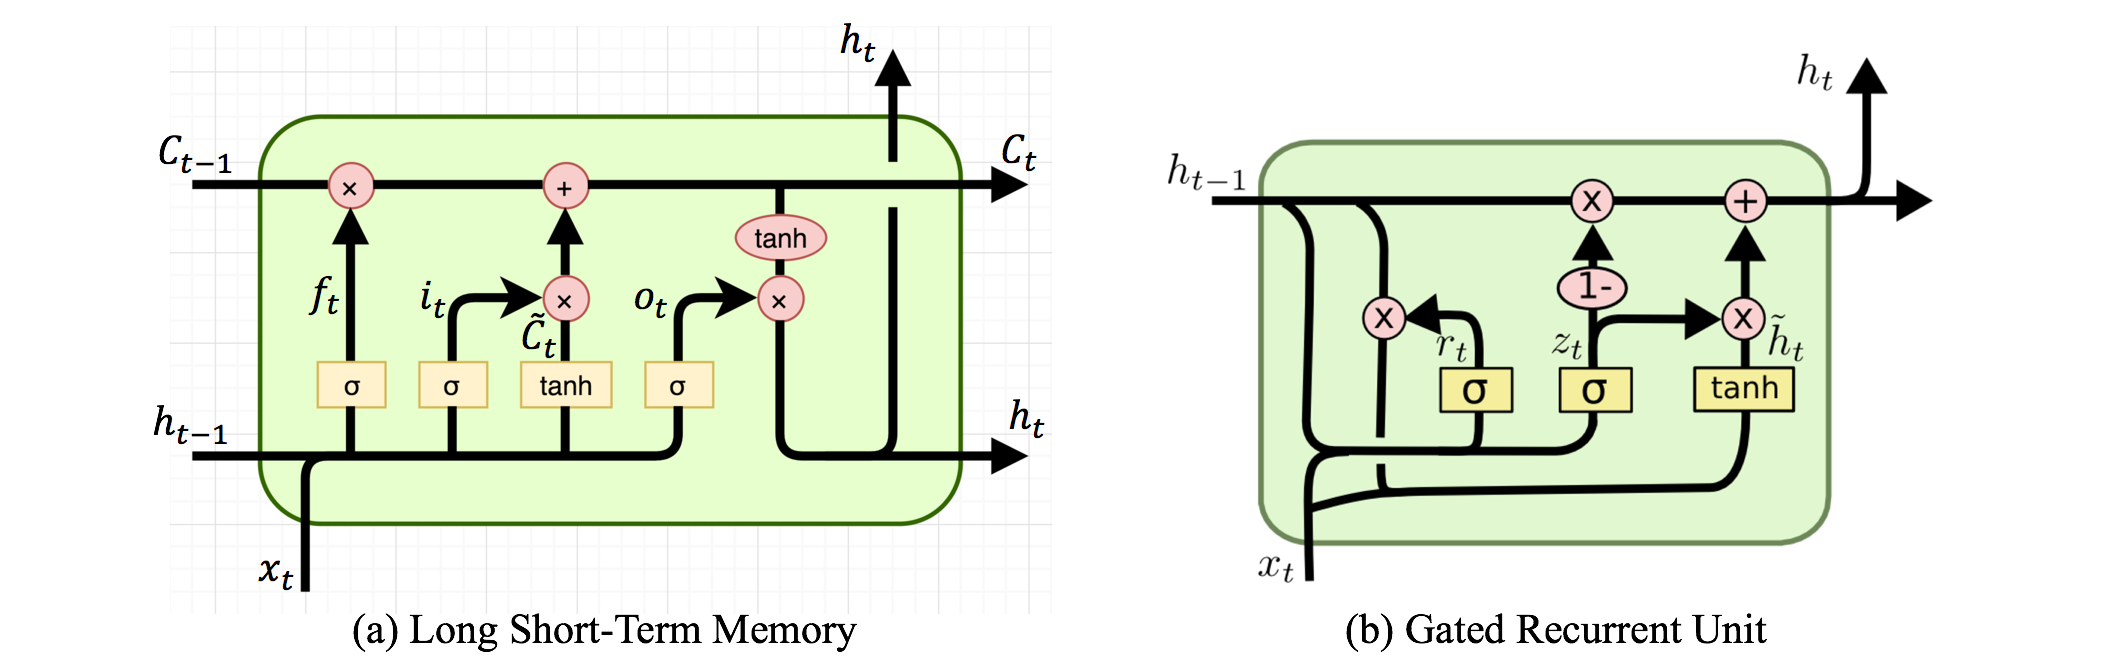
\includegraphics[width=15cm]{GRU-LSTM.png}

Gradient Recurrent Unit:

$$\tilde{c}^{<t>} = tanh( W_c [ \Gamma_r * c^{<t-1>},x^{<t>}] + b_c)$$
$$ \Gamma_u = \sigma(W_u[c^{<t-1>},x^{<t>}] + b_u)$$
$$ \Gamma_r = \sigma(W_r[c^{<t-1>},x^{<t>}] + b_r)$$
$$c^{<t>} = \Gamma_u * \tilde{c}^{<t>} + (1 - \Gamma_u) * c^{<t-1>}$$
$$a^{<t>} = c^{<t>}$$

Long Short Term Memory:

$$\tilde{c}^{<t>} = tanh( W_c [ c^{<t-1>},x^{<t>}] + b_c)$$
$$ \Gamma_u = \sigma(W_u[c^{<t-1>},x^{<t>}] + b_u)$$
$$ \Gamma_f = \sigma(W_f[c^{<t-1>},x^{<t>}] + b_r)$$
$$\Gamma_o = \sigma(W_o[c^{<t-1>},x^{<t>}] + b_o)$$
$$c^{<t>} = \Gamma_u * \tilde{c}^{<t>} + \Gamma_f * c^{<t-1>}$$
$$a^{<t>} = \Gamma_o c^{<t>}$$

\section{Bidirectional RNN and Deep RNN}

Bidirectional RNN - Two activations connected in two different directions

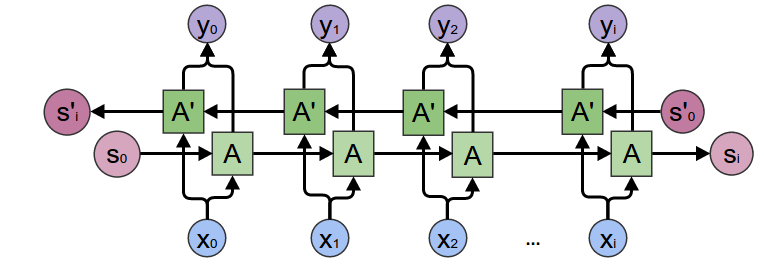
\includegraphics[width=15cm]{Bidirectional.png}

Deep RNN - Stacking RNN Layers together. Three layers are already pretty deep.

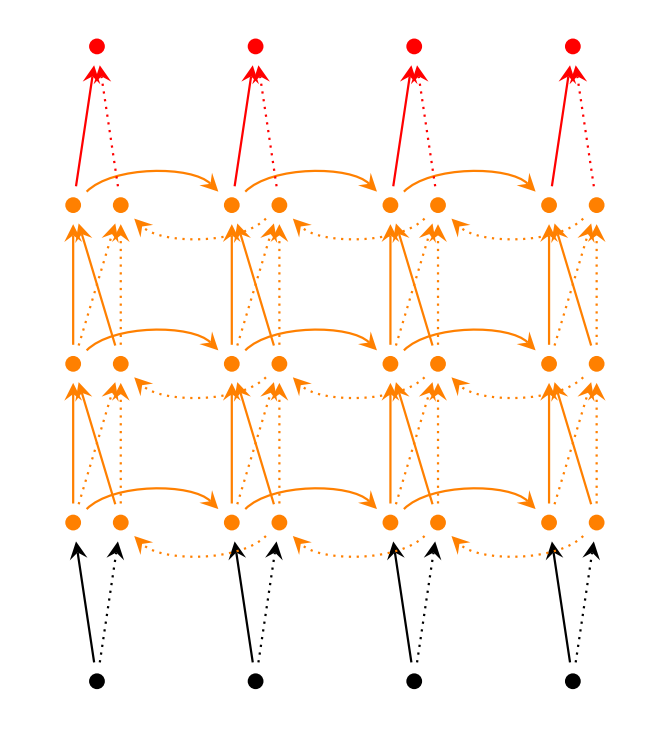
\includegraphics[width=15cm]{DeepRNN.png}

\section{Language Model}

Language model uses data from a \textbf{Corpus}. it models probabilities of words appear(generative model).

The input is a language sequence, prediction is the (conditional) probability of next word appearing. The prediction is a Sampling (according to predicted probability until we hit EOS).

Application examples like;

Sentiment Classification:

$$\text{word embedding} \rightarrow Average \rightarrow softmax \rightarrow \hat{y}$$

Or a \textit{many to one} RNN with sentiment as the (only) output at the last step.

\chapter{Generative Adversarial Networks(GAN)}
	
\chapter{Reinforcement Learning}
 
\end{document}                          % The required last line 